\documentclass[11pt,a4paper]{article}
\usepackage[margin=2.4cm]{geometry}
\usepackage[T1]{fontenc}
\usepackage{lmodern}
\usepackage{amsmath,amssymb}
\usepackage{booktabs}
\usepackage{multirow}
\usepackage{float}
\usepackage{graphicx}
\usepackage{siunitx}
\usepackage{microtype}
\usepackage{xcolor}
\usepackage{pgfplots}
\pgfplotsset{compat=1.18}
\usetikzlibrary{positioning,arrows.meta,calc}
\usepackage[hidelinks]{hyperref}
\sisetup{group-separator={,},group-minimum-digits=4}
\newcommand{\cfg}[1]{\texttt{#1}}
\setlength{\parskip}{0.3em}
\setlength{\emergencystretch}{2em}
\definecolor{s1}{HTML}{2a78d6}
\definecolor{s2}{HTML}{eb6834}
\definecolor{s3}{HTML}{1baf7a}
\definecolor{inkmuted}{HTML}{6b6a64}

\begin{document}

\begin{center}
  {\LARGE End-to-end sonar pipeline on the\\[0.2em]
  Raspberry Pi~4 and Pi~2}\\[0.6em]
  {\large Laboratory report, project \texttt{sonar\_edge} (milestones M8--M10)}\\[0.3em]
  21 November 2026
\end{center}
\vspace{0.3em}

\begin{abstract}
\noindent
The marine-debris detector of this project ran in C only from a
$360 \times 240$ image that Python had already resized, and it returned
boxes in network pixels. This report extends the C program to the whole
path from the sonar software's fan image to the outputs. A lookup-table
front end resizes the native $320 \times 480$ fan image exactly as in
training; one network pass gives boxes, class names, probabilities and a
segmentation mask; boxes are mapped back into the fan image and to range
and bearing; and a command-line tool writes one JSON line per frame. The
pipeline was run over a full test fold of 439 frames on a Raspberry Pi~4
and on a 32-bit Raspberry Pi~2, to which the NEON kernel was ported. On
both boards the output equals the laptop's on every frame, so the mAP is
identical (63.81 with the deployed model). A frame takes 21.9~ms on the
Pi~4 and 128.5~ms on the Pi~2, of which the front end is 6\,\% and 4\,\%.
A path for raw polar beam data is implemented as well. The tank dataset
holds only projected fan images, so on that data the path was tested on
frames back-projected from those images. It was then run on 28 native ARIS
recordings of plastic litter from a public river dataset. There the reader
and geometry match independent projections, and the Pi~4 needs 21.1~ms per
frame. The detector does not transfer, however: it responds to riverbed
texture as often without plastic as with it, and these recordings have no
labels for an accuracy figure.

For the edge task, detection on a small underwater vehicle at the sonar's
frame rate, the recordings were streamed at 15 frames/s from a laptop
over Ethernet to the boards for 30 minutes each. The fanless Pi~4 kept up
on one core (0.03\,\% of frames dropped, result 30~ms after capture,
57\,$^\circ$C at most, no throttling); the Pi~2 kept up on three cores,
with each result 145~ms after capture. A network trained on the polar
(beam $\times$ range) form of the images instead of the fan image was
6.5 points worse at equal compute, so the fan-image input stays.
\end{abstract}

% ===========================================================================
\section{Aim}

To turn the verified int8 detector into a program that takes a sonar frame
as the sonar software delivers it and returns detections, a mask and their
positions in sonar coordinates, entirely in C, and to show on two
Raspberry Pi boards that this program reproduces the reference results
exactly and to measure what each stage costs.

\paragraph{Edge task.} The target is onboard debris detection on a small
ROV or AUV. The sonar delivers frames at its own rate, 15 frames/s for the
ARIS~3000 recordings used here, and the vehicle's link cannot carry sonar
video: one raw frame is 53--124~KB, up to 1.9~MB/s. The detector must keep
up with the sensor on the vehicle's computer and send only its results. The
system is treated as an image-to-image pipeline: the sonar software's fan
image goes in, detections and a mask come out. Talking to a live sonar over
its own network protocol is outside the scope.

The objectives were:
\begin{enumerate}
  \item a front end that resizes the native fan image bit-exactly as in
        training, and a second one for raw polar beam data;
  \item one network pass for both boxes and mask;
  \item outputs in fan-image pixels and in range and bearing;
  \item the 32-bit Raspberry Pi~2 as a second target, which needed a port
        of the NEON kernel;
  \item an on-device test over a full test fold: identity with the laptop,
        accuracy, and the time of every stage;
  \item operation on a live stream at the sonar's frame rate, emulated by
        replaying recordings over the network, including a 30-minute run per
        board;
  \item a check whether the network should take the polar (beam $\times$
        range) form of the data instead of the fan image.
\end{enumerate}

% ===========================================================================
\section{Background}

The project (\texttt{report/project\_report.pdf}, milestones M0--M7)
trained a one-stage, anchor-free detector for ten debris classes and the
tank walls on the 1\,868 frames of the public ARIS Explorer~3000
water-tank dataset. Frames were grouped into 191 scenes and evaluated by
five-fold scene cross-validation. The deployed network, \cfg{small} at
$360 \times 240$ (\num{42463} parameters, 78~M multiply--accumulates),
reaches 52.3~$\pm$~1.7 pooled mAP@0.5 measured on the Pi~4. It is
quantised to 8-bit integers and run by a dependency-free C11 runtime that
is bit-exact with the Python integer reference; a hand-written NEON kernel
brings it to 20.3~ms per frame on one Cortex-A72 core. A variant with a
segmentation head (\cfg{small\_360\_segdice}, ``\cfg{segdice}'' below)
also predicts a class label per output cell, at some cost in box mAP.

Until this milestone the C program covered only the network and the box
decoder: the resize to the network input was done in Python, and the
mask needed a second network pass.

% ===========================================================================
\section{The pipeline}
\label{sec:pipeline}

Figure~\ref{fig:pipeline} shows the pipeline. Every stage runs in C, in
static memory, with no dependencies.

\begin{figure}[H]
\centering
\resizebox{\textwidth}{!}{%
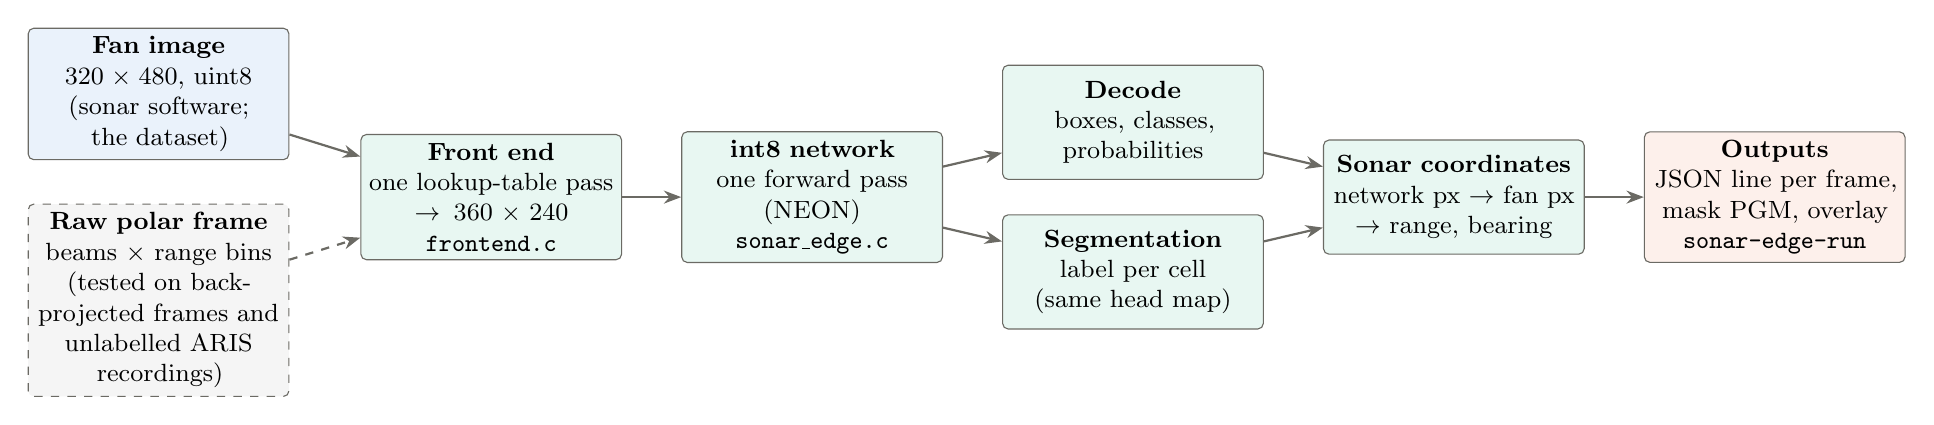
\begin{tikzpicture}[
  box/.style={draw=inkmuted, rounded corners=2pt, align=center, font=\small, text width=3.1cm, minimum height=1.45cm, inner sep=3pt},
  inp/.style={box, fill=s1!10},
  syn/.style={box, fill=gray!8, dashed},
  stage/.style={box, fill=s3!10},
  outp/.style={box, fill=s2!10},
  arr/.style={-{Stealth[length=2.2mm]}, inkmuted, thick},
  node distance=0.55cm and 0.75cm,
]
\node[inp] (fan) {\textbf{Fan image}\\$320 \times 480$, uint8\\(sonar software;\\the dataset)};
\node[syn, below=of fan] (pol) {\textbf{Raw polar frame}\\beams $\times$ range bins\\(tested on back-\\projected frames and\\unlabelled ARIS\\recordings)};
\coordinate (mid) at ($(fan.east)!0.5!(pol.east)$);
\node[stage, right=0.9cm of mid] (fe) {\textbf{Front end}\\one lookup-table pass\\$\rightarrow 360 \times 240$\\\texttt{frontend.c}};
\node[stage, right=of fe] (net) {\textbf{int8 network}\\one forward pass\\(NEON)\\\texttt{sonar\_edge.c}};
\node[stage, right=of net, yshift=0.95cm] (dec) {\textbf{Decode}\\boxes, classes,\\probabilities};
\node[stage, right=of net, yshift=-0.95cm] (seg) {\textbf{Segmentation}\\label per cell\\(same head map)};
\node[stage, right=of dec, yshift=-0.95cm] (crd) {\textbf{Sonar coordinates}\\network px $\rightarrow$ fan px\\$\rightarrow$ range, bearing};
\node[outp, right=of crd] (out) {\textbf{Outputs}\\JSON line per frame,\\mask PGM, overlay\\\texttt{sonar-edge-run}};
\draw[arr] (fan) -- (fe);
\draw[arr, dashed] (pol) -- (fe);
\draw[arr] (fe) -- (net);
\draw[arr] (net) -- (dec);
\draw[arr] (net) -- (seg);
\draw[arr] (dec) -- (crd);
\draw[arr] (seg) -- (crd);
\draw[arr] (crd) -- (out);
\end{tikzpicture}}
\caption{The end-to-end C pipeline. Solid input: the form in which the
dataset and the sonar software provide frames, tested exactly. Dashed
input: raw beam data, tested on frames back-projected from the dataset's
fan images and on unlabelled native ARIS recordings from another dataset
(Section~\ref{sec:dans}).}
\label{fig:pipeline}
\end{figure}

\noindent\fbox{\begin{minipage}{\dimexpr\linewidth-2\fboxsep-2\fboxrule}
\textbf{What the input is.} The dataset contains only Cartesian fan images,
already projected from the beams by the sonar software; it has no raw
(polar) ARIS data. The fan path of the pipeline starts from those images,
at their native $320 \times 480$, and is the one whose accuracy is
reported. The polar path is implemented, but on this data it was tested
only on frames \emph{we} made by sampling the fan images back onto a
128-beam $\times$ 439-bin grid (\texttt{src/sonar\_edge/polar.py}). Those
frames carry the fan image's interpolation and none of a real sonar's beam
pattern, so they test the remap code, not performance on raw recordings.
The dataset gives no metric scale either, so ranges for the tank data are
reported in pixels.

The polar path was then also run on native ARIS recordings from a
different public dataset (Section~\ref{sec:dans}). Those recordings test
the raw-data path on real sonar data, but they have no labels. Detection
accuracy on raw data therefore remains unmeasured.
\end{minipage}}

\subsection{Front end}

A lookup table is built once at start-up; each frame then takes one
integer pass from the input to the network's $360 \times 240$ uint8
input. The tables take 873~KB of static memory.

In \emph{fan} mode the native image is resized exactly as in training.
For $360 \times 240$ the training pipeline uses Pillow's box filter, so
its arithmetic is reproduced: weights computed and normalised as Pillow
computes them, held with 22 fraction bits, a horizontal pass and then a
vertical pass. The $240 \times 160$ models are trained with a float32
block mean and round-half-to-even instead; that depends only on the block
sum and becomes a table.

In \emph{polar} mode the input is raw beam data, range bins (near to far)
by beams. Each network pixel is mapped through the fan geometry to a
fractional (range bin, beam) position and interpolated bilinearly with
8-bit weights. Beam angles are uniform over the field of view or come
from a per-beam table; points outside the fan read 0, like the black
corners of a fan image.

The fan geometry was fitted to the fan edges and arcs of all 1\,868
frames (Table~\ref{tab:fangeom}); the fitted field of view agrees with
the ARIS Explorer~3000 specification.

\begin{table}[H]
\centering
\caption{Fan geometry of the dataset's images (\texttt{se\_fan\_watertank}).}
\label{tab:fangeom}
\begin{tabular}{ll}
\toprule
Quantity & Value \\
\midrule
Apex (sonar position) $(u, v)$ & (160.0, 602.7) px, below the image \\
Field of view & \SI{30.0}{\degree} (fit 30.07; ARIS 3000 specification 30) \\
Near / far radius & 138.6 / 578.0 px from the apex (residuals $\le 1$ px) \\
Metres per pixel & unknown: ranges in pixels \\
\bottomrule
\end{tabular}
\end{table}

\subsection{One pass, sonar coordinates and the tool}

\texttt{se\_process} runs the network once and derives both outputs from
the same head map: the detections, with the decoder, threshold and
top-$K$ of the earlier \texttt{se\_detect}, and the label map. Emitting
both used to cost two network passes. Each box is then mapped from
network pixels back to fan-image pixels by the inverse of the resize, and
its centre gives a range (distance from the apex) and a bearing (angle
from the centre line, positive to the right).

The command-line tool \texttt{sonar-edge-run} reads PGM files at network
size or at fan size, or raw polar frames from a file or standard input.
For every frame it writes one JSON line with the time of each stage, each
detection's class name, logit, probability, box in network and fan
pixels, range and bearing, and the label count per class; optionally it
also writes the label map and an overlay of boxes and mask on the fan
image. Two models were exported: the deployed \cfg{small}
$360 \times 240$ (fold~0 network, boxes only) and \cfg{segdice}
(stride-4 head with Dice term, fold~0, boxes and mask).

% ===========================================================================
\section{Boards and the 32-bit port}
\label{sec:boards}

\begin{table}[H]
\centering
\caption{The two target boards. Both were used without fan or heat sink.}
\label{tab:hw}
\resizebox{\textwidth}{!}{%
\begin{tabular}{lll}
\toprule
 & Raspberry Pi~4 B & Raspberry Pi~2 B \\
\midrule
Processor & BCM2711, 4 $\times$ Cortex-A72, \SI{1.8}{GHz} & BCM2836, 4 $\times$ Cortex-A7, \SI{900}{MHz} \\
Instruction set & 64-bit ARMv8.0, NEON (32 vector registers) & 32-bit ARMv7, NEON + VFPv4 (16 vector registers) \\
Memory & 4 GB; \SI{32}{KB} L1D per core, \SI{1}{MB} shared L2 & 1 GB \\
OS / compiler & Debian 13, kernel 6.18, gcc 14.2 & Raspbian 13 (armhf), kernel 6.18, gcc 14.2 \\
\bottomrule
\end{tabular}}
\end{table}

\paragraph{Port.} The NEON kernel multiplies an activation broadcast from
one vector lane against 16 int16 weights. It used intrinsics that exist
only in 64-bit mode: the by-element multiply on a 128-bit vector
(\texttt{vmlal\_laneq\_s16}) and the \texttt{\_high\_} forms. Three macros
now express it for both modes; on AArch32 the element is taken from the
matching 64-bit half of the activation vector, which gives the same
products and sums, so the result is still exact by construction. The
64-bit code is unchanged: after the port the Pi~4 build passes the golden
test, gives byte-identical full-fold output for all four models, and runs
at the same speed (8.9 / 20.2 / 46.2 / 91.6~ms against 9.0 / 20.3 / 46.5 /
91.8 before). Raspbian's compiler targets ARMv6 without NEON by default,
so the Pi~2 build adds \texttt{-mcpu=cortex-a7 -mfpu=neon-vfpv4}.

\paragraph{Pi~2 benchmark.} The network-only benchmark of the Pi~4 was
repeated on the Pi~2 with four builds per model (Table~\ref{tab:pi2}).
All 16 builds passed the golden test, and the four-pixel build's output
on the 439 test-fold frames was byte-identical to the Pi~4's for all four
models. A first attempt failed because the board's power supply was too
weak: large network packets were lost and the firmware's under-voltage
flag was set. With a stronger supply the throttle flags read 0x0 for
every run, at \SI{39}{}--\SI{54}{\celsius}.

\begin{table}[H]
\centering
\caption{Raspberry Pi~2, network only, ms per frame on one core (mean of
three repeats of about 25~s, NEON repeats within 1\,\%). ARMv6:
Raspbian's default target; A7: scalar for the Cortex-A7. ``4 copies'':
four independent processes, fastest NEON build (bold). Last column: Pi~4,
four-pixel NEON.}
\label{tab:pi2}
\footnotesize
\setlength{\tabcolsep}{3.5pt}
\begin{tabular}{lrrrrrrrrr}
\toprule
 & \multicolumn{4}{c}{Pi~2, one core (ms)} & NEON vs & \multicolumn{2}{c}{Pi~2, 4 copies} & Peak & Pi~4 \\
\cmidrule(lr){2-5}\cmidrule(lr){7-8}
Model & ARMv6 & A7 & NEON 1 px & NEON 4 px & scalar A7 & fps & ms/copy & memory & ms \\
\midrule
\cfg{small} $240{\times}160$ & 295.1 & 288.8 & \textbf{54.8} & 56.3 & 5.3$\times$ & 69.8 & 56--57 & 1.8 MB & 9.0 \\
\textbf{\cfg{small} $360{\times}240$} & 663.8 & 650.0 & \textbf{124.5} & 126.8 & 5.2$\times$ & \textbf{30.7} & 126--130 & 2.3 MB & 20.3 \\
\cfg{small\_wide} $360{\times}240$ & 1565.8 & 1555.0 & 392.2 & \textbf{315.6} & 4.9$\times$ & 12.0 & 330--334 & 2.5 MB & 46.5 \\
\cfg{wide} $480{\times}320$ & 3418.8 & 3384.0 & 798.7 & \textbf{649.6} & 5.2$\times$ & 5.8 & 680--689 & 3.3 MB & 91.8 \\
\bottomrule
\end{tabular}
\end{table}

NEON is about five times faster than scalar code on the Cortex-A7
(6.2--7.1 times on the Pi~4), and targeting the A7 instead of ARMv6 gains
scalar code only 1--2\,\%. The four-pixel kernel, which reuses each
weight load for four output pixels, needs 22 vector registers; with 16 it
spills. On the 32-channel models the spills cost slightly more than the
saved weight loads (2--3\,\% slower), while on the 64-channel models the
saved weight traffic dominates (23--24\,\% faster), the same pattern as
on the Pi~4. Four independent copies reach 94--96\,\% of four times the
one-core rate, better than the Pi~4's 32-channel runs. Overall the Pi~2 is
6.1--7.1 times slower than the Pi~4: the deployed model takes 124.5~ms
(8 frames/s) on one core and reaches 30.7 frames/s with four frames in
flight.

% ===========================================================================
\section{On-device test of the pipeline}
\label{sec:method}

Test fold~0 (439 frames) was used in two forms: the native
$320 \times 480$ fan images, and the same frames back-projected to polar.
Every board built the committed source natively, passed \texttt{make
test} (network against the Python reference) and \texttt{make
test-frontend} (front end against the Python resize), and then ran
\texttt{sonar-edge-run} over the fold for both models. The output was
compared with the laptop's: the JSON with the timing fields removed, and
the label maps byte for byte. The detections were scored with the
project's Python metric. Timings are means over the fold, one call per
frame, with the temperature and throttle flags read before and after
each run. On the Pi~2 both NEON kernels were run.

% ===========================================================================
\section{Results}
\label{sec:results}

\subsection{Exactness}

On the laptop the fan front end reproduced the Python resize on all
1\,868 frames, at $360 \times 240$ and at $240 \times 160$. On the boards
every model, input mode and kernel reproduced the laptop on every frame
(Table~\ref{tab:e2eid}), and both test programs passed for every build.
The pipeline therefore adds no error of its own, and its mAP is the same
on every machine.

\begin{table}[H]
\centering
\caption{Test fold~0, 439 frames: frames whose pipeline output equals the
laptop's (JSON without timing fields; label maps byte for byte).
$^\dagger$Polar input back-projected from the fan images, not raw sonar
data.}
\label{tab:e2eid}
\begin{tabular}{llcccc}
\toprule
 & & \multicolumn{2}{c}{\cfg{small}: JSON} & \multicolumn{2}{c}{\cfg{segdice}: JSON / masks} \\
\cmidrule(lr){3-4}\cmidrule(lr){5-6}
Board & Build & fan & polar$^\dagger$ & fan & polar$^\dagger$ \\
\midrule
Raspberry Pi~4 & AArch64, NEON 4 px & 439 & 439 & 439 / 439 & 439 / 439 \\
Raspberry Pi~2 & ARMv7, NEON 1 px & 439 & 439 & 439 / 439 & 439 / 439 \\
Raspberry Pi~2 & ARMv7, NEON 4 px & 439 & 439 & 439 / 439 & 439 / 439 \\
\bottomrule
\end{tabular}
\end{table}

\subsection{Accuracy}

\begin{table}[H]
\centering
\caption{Box mAP@0.5 (\%) of the pipeline on test fold~0, identical on the
laptop, the Pi~4 and the Pi~2 (both kernels). Single fold, single seed:
not comparable with the pooled five-fold figures of the project report.}
\label{tab:e2emap}
\begin{tabular}{lcc}
\toprule
Model & Fan input (native $320 \times 480$) & Polar input (back-projected) \\
\midrule
\cfg{small} $360{\times}240$ & 63.81 & 63.17 \\
\cfg{segdice} & 57.09 & 52.32 \\
\bottomrule
\end{tabular}
\end{table}

The fan-input figures equal those of the Python integer model on
pre-resized frames (63.81; 57.08 for \cfg{segdice}, the 0.01 coming from
the order of tied scores), which confirms that the C resize is exact.
The back-projected polar input costs \cfg{small} 0.6 points and
\cfg{segdice} 4.8 points; the laptop gives the same figures, so this is a
property of the models on resampled images, not of a device.

\subsection{Time per stage}

\begin{table}[H]
\centering
\caption{Pipeline time per frame, ms, mean over the 439 frames, one core.
Pi~2: single-pixel kernel (the four-pixel kernel totals 132.4 / 131.1 /
140.1 / 139.0~ms in the same row order).}
\label{tab:e2etime}
\resizebox{\textwidth}{!}{%
\begin{tabular}{lllrrrrr}
\toprule
Board & Model & Input & Front end & Network & Decode & Segmentation & Total \\
\midrule
Raspberry Pi~4 & \cfg{small} & fan & 1.40 & 20.14 & 0.37 & -- & \textbf{21.90} \\
               & \cfg{small} & polar (back-projected) & 0.53 & 20.07 & 0.36 & -- & 20.96 \\
               & \cfg{segdice} & fan & 1.40 & 21.20 & 0.40 & 0.24 & \textbf{23.24} \\
               & \cfg{segdice} & polar (back-projected) & 0.54 & 21.56 & 0.40 & 0.24 & 22.74 \\
\midrule
Raspberry Pi~2 & \cfg{small} & fan & 5.44 & 121.91 & 1.15 & -- & \textbf{128.50} \\
               & \cfg{small} & polar (back-projected) & 2.85 & 121.66 & 1.15 & -- & 125.65 \\
               & \cfg{segdice} & fan & 5.44 & 127.71 & 1.27 & 2.15 & \textbf{136.56} \\
               & \cfg{segdice} & polar (back-projected) & 2.82 & 127.32 & 1.27 & 2.15 & 133.56 \\
\bottomrule
\end{tabular}}
\end{table}

\begin{figure}[H]
\centering
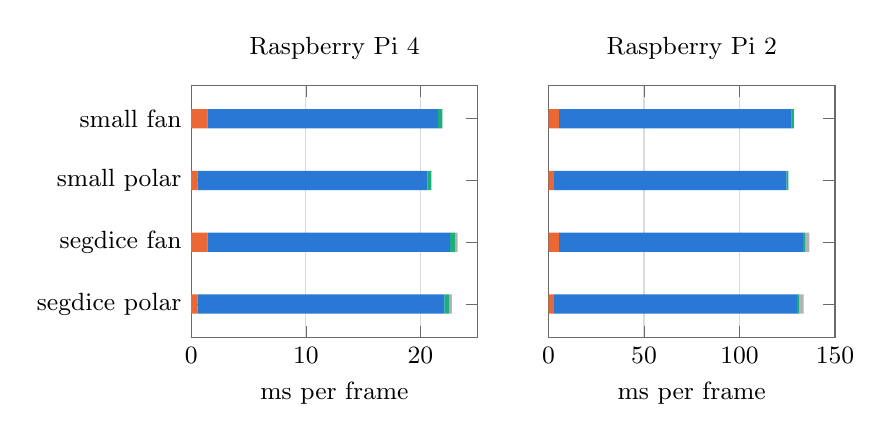
\begin{tikzpicture}
\pgfplotsset{e2ebar/.style={
  xbar stacked, bar width=7pt, scale only axis, width=0.3\textwidth, height=3.2cm,
  xlabel={ms per frame}, ytick=data, enlarge y limits=0.18,
  symbolic y coords={segdice polar,segdice fan,small polar,small fan},
  title style={font=\small}, axis line style={inkmuted}, tick style={inkmuted},
  ticklabel style={font=\small}, label style={font=\small},
  xmajorgrids, grid style={inkmuted!25}}}
\begin{axis}[e2ebar, name=a1, xmin=0, xmax=25, title={Raspberry Pi~4},
  legend to name=e2eleg, legend columns=4, legend style={draw=none, font=\small, /tikz/every even column/.append style={column sep=0.6em}}]
\addplot[fill=s2, draw=none] coordinates {(1.40,small fan) (0.53,small polar) (1.40,segdice fan) (0.54,segdice polar)};
\addplot[fill=s1, draw=none] coordinates {(20.14,small fan) (20.07,small polar) (21.20,segdice fan) (21.56,segdice polar)};
\addplot[fill=s3, draw=none] coordinates {(0.37,small fan) (0.36,small polar) (0.40,segdice fan) (0.40,segdice polar)};
\addplot[fill=gray!60, draw=none] coordinates {(0,small fan) (0,small polar) (0.24,segdice fan) (0.24,segdice polar)};
\legend{front end, network, decode, segmentation}
\end{axis}
\begin{axis}[e2ebar, at={($(a1.east)+(0.9cm,0)$)}, anchor=west, xmin=0, xmax=150, title={Raspberry Pi~2}, yticklabels={}]
\addplot[fill=s2, draw=none] coordinates {(5.44,small fan) (2.85,small polar) (5.44,segdice fan) (2.82,segdice polar)};
\addplot[fill=s1, draw=none] coordinates {(121.91,small fan) (121.66,small polar) (127.71,segdice fan) (127.32,segdice polar)};
\addplot[fill=s3, draw=none] coordinates {(1.15,small fan) (1.15,small polar) (1.27,segdice fan) (1.27,segdice polar)};
\addplot[fill=gray!60, draw=none] coordinates {(0,small fan) (0,small polar) (2.15,segdice fan) (2.15,segdice polar)};
\end{axis}
\end{tikzpicture}\\[0.4em]
\ref{e2eleg}
\caption{Pipeline time per frame by stage (Table~\ref{tab:e2etime}; note
the different scales). ``polar'' rows use back-projected frames. The
network is 92--97\,\% of the total on both boards.}
\label{fig:e2etime}
\end{figure}

On the Pi~4 a native fan frame becomes boxes, classes and sonar
coordinates in 21.9~ms with the deployed model, or 23.2~ms with the mask:
the fan front end adds 1.4~ms (6\,\%) and the mask 0.24~ms. The fan front
end is slower than the polar one (1.40 against 0.53~ms) because the box
filter combines several source pixels per output pixel in two passes,
against one bilinear point in polar mode; both loops are scalar. On the
Pi~2 the pipeline takes 128.5~ms, or 136.6~ms with the mask, and the
single-pixel kernel is 3--4~ms faster than the four-pixel one, as in the
network-only benchmark. The boards ran at \SI{53}{}--\SI{58}{\celsius}
(Pi~4) and \SI{41}{}--\SI{43}{\celsius} (Pi~2), and
\texttt{get\_throttled} read 0x0 before and after every run.

\subsection{Test on real raw ARIS recordings (DANS dataset)}
\label{sec:dans}
Because the tank dataset has no raw data, the polar path was also run on
native ARIS recordings from a different public dataset: \emph{Detection of
plastic litter using an ARIS sonar} (Radboud University, 2021; DANS,
doi:10.17026/dans-xee-n9rq, CC~BY~4.0). It holds 71 public \texttt{.aris}
files of plastic objects (containers, pieces, cups, a rim) and control
recordings in the river Waal. 28 recordings were used: the 23 of the
16~April session and 6 of the 19~April session, less one duplicate. All
come from an ARIS Explorer 3000 with 128 beams at 15~frames/s (13.7 for the
longest window); the range windows start at 0.70~m and end at 1.86--4.75~m.
Up to 200 frames were taken from each recording (every $N$-th frame), 4\,780
per model.

\paragraph{Reader and geometry.} A C reader (\texttt{runtime/aris.c})
follows the file format of Sound Metrics' \texttt{aris-file-sdk}: a
1024-byte file header, then per frame a 1024-byte header and the samples
$\times$ beams data. ARIS stores beam~0 at the right, so the reader flips the
beam order, and it takes each beam's angle from the SDK's ARIS~3000 tables
(MIT licence) instead of assuming uniform spacing. The range window comes
from each frame's sample delay, sample period and sound speed. The rendered
images were checked against two independent projections: one written from
the SDK's formulas, which agrees within one grey level (98.5\,\% of pixels
identical), and the third-party reader pyARIS, which correlates at 0.984
after a $5 \times 5$ blur (0.93 unblurred). The mirrored image correlates at
0.49, which confirms the beam order. Each recording is drawn in its true fan
shape, with the far edge of the window on the training fan's far radius
(578~px). This gives a metric scale for these data (window end / 578~px, for
example 5.3~mm/px for a 3.08~m window), so ranges are reported in metres.
Objects therefore appear at a different pixel size from the tank, depending
on the window.

\paragraph{Equality and cost.} On the Pi~4 the output for all 195 frames of
the \emph{PlasticContainer} recording equals the laptop's for both models.
Table~\ref{tab:danstime} gives the time per stage. The front end costs the
same as on back-projected frames (0.55 against 0.53~ms), so a real 15~frames/s
ARIS stream needs about a third of one Pi~4 core.

\begin{table}[H]
\centering
\caption{Time per frame on real ARIS recordings, ms (10 frames $\times$ 20
repeats). Pi~4: \SI{57.4}{\celsius} before, \SI{55.0}{\celsius} after,
\texttt{get\_throttled} 0x0.}
\label{tab:danstime}
\begin{tabular}{llrrrrr}
\toprule
Model & Machine & Front end & Network & Decode & Mask & Total \\
\midrule
small@360 & laptop & 0.10 & 20.30 & 0.11 & -- & 20.50 \\
          & Pi~4   & 0.55 & 20.14 & 0.37 & -- & 21.06 \\
segdice   & laptop & 0.10 & 20.31 & 0.11 & 0.04 & 20.56 \\
          & Pi~4   & 0.55 & 21.20 & 0.41 & 0.24 & 22.40 \\
\bottomrule
\end{tabular}
\end{table}

\paragraph{What the detector does on river data.} The recordings have no
labels, so no accuracy can be computed. Table~\ref{tab:danshits} counts
the frames with at least one detection at probability $\ge 0.3$.

\begin{table}[H]
\centering
\caption{Frames with a detection at $p \ge 0.3$, by group of recordings.
Almost all detections are ``Chain'', a few ``Wall''.}
\label{tab:danshits}
\begin{tabular}{lrrrr}
\toprule
Recordings & Window end (m) & Frames & small@360 & segdice \\
\midrule
Controls, no plastic (2)        & 1.87--1.89 & 334   & 133 (40\,\%) & 192 (57\,\%) \\
Containers (6)                  & 1.86--3.08 & 1\,019 & 341 (33\,\%) & 357 (35\,\%) \\
Pieces and rim (8)              & 1.89--2.50 & 1\,412 & 336 (24\,\%) & 894 (63\,\%) \\
Cups (6)                        & 1.89       & 1\,024 & 460 (45\,\%) & 1\,012 (99\,\%) \\
19~April session (6)            & 3.51--4.75 & 991   & 0            & 0 \\
\midrule
All (28)                        &            & 4\,780 & 1\,270 (27\,\%) & 2\,455 (51\,\%) \\
\bottomrule
\end{tabular}
\end{table}

\begin{figure}[H]
\centering
\begin{minipage}{0.24\textwidth}\centering
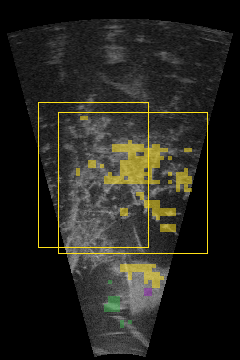
\includegraphics[width=\linewidth]{fig/dans_container.png}\\[-0.2em]
{\small (a) PlasticContainer2}
\end{minipage}\hfill
\begin{minipage}{0.24\textwidth}\centering
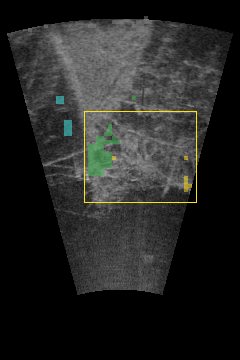
\includegraphics[width=\linewidth]{fig/dans_control.png}\\[-0.2em]
{\small (b) Weight\_control}
\end{minipage}\hfill
\begin{minipage}{0.24\textwidth}\centering
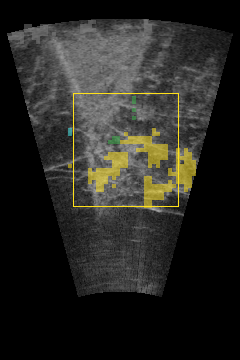
\includegraphics[width=\linewidth]{fig/dans_cup.png}\\[-0.2em]
{\small (c) Cup}
\end{minipage}\hfill
\begin{minipage}{0.24\textwidth}\centering
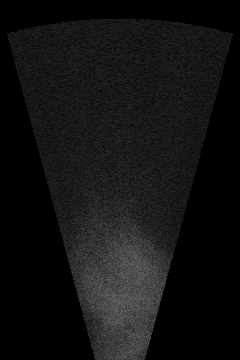
\includegraphics[width=\linewidth]{fig/dans_river.png}\\[-0.2em]
{\small (d) vegContainer}
\end{minipage}
\caption{Real ARIS frames through the pipeline (segdice model: boxes at
$p \ge 0.3$ and mask cells). (a) A plastic-container recording (frame 843)
and (b) a control without plastic (frame 180): both give ``Chain'' boxes and
mask cells on textured riverbed. (c) A cup recording (frame 322): the
same response. (d) A 4.75~m river recording (frame 210): no detections.
The plastic objects could not be located by eye in these frames.}
\label{fig:dans}
\end{figure}

The models do not transfer from the tank to the river. The detections
fire on textured bed and vegetation, mostly as ``Chain''. They are as
frequent in the control recordings without plastic as in the recordings
with it: 133 of 196 frames of the \emph{PinAlone} control for small@360,
185 of 196 for segdice. The rate depends on the recording set and range
window more than on the presence of plastic. The plastic objects could not
be located by eye, so it is unknown whether any box lands on one. The six
longer-range recordings of 19~April give no detections at all.

This test therefore validates the raw-data path on real ARIS recordings:
the reader, the beam geometry, the front end, the metric ranges, exactness
on the device and the real-time cost. It does \emph{not} measure detection
accuracy on raw data, and it is no evidence that the detector works in the
field. That would need labelled recordings from the target environment and
fine-tuning on them.

\subsection{Polar input instead of the fan image}
\label{sec:polar}

The network could also take the sonar's native form, beams $\times$ range
bins, and skip the front end. To test this, every fan frame of the dataset
was sampled back onto a polar grid of 440 range bins and 128 or 192 beams
(back-projected frames, as in Section~\ref{sec:pipeline}). The ground-truth
boxes were converted through the masks: a box taken to polar form and back
overlaps the original with median IoU 0.84, and these converted boxes,
used as perfect detections, score 98.9 mAP, so the conversion costs at most
about one point. \cfg{small} was trained with the same recipe, folds and
three seeds as the deployed model, and its detections were mapped back to
the fan image and scored against the original boxes
(Table~\ref{tab:polar}).

\begin{table}[H]
\centering
\caption{Fan-image input against back-projected polar input: pooled
five-fold mAP@0.5 in fan-image space, mean $\pm$ s.d.\ over three seeds,
and the paired difference over the 15 fold--seed pairs.}
\label{tab:polar}
\begin{tabular}{lrcrc}
\toprule
Input & MACs & Pooled mAP & Paired difference & Better / worse \\
\midrule
fan image $360 \times 240$ (deployed) & 78.4~M & \textbf{52.6~$\pm$~1.9} & -- & -- \\
polar $440 \times 128$ (back-projected) & 51.1~M & 45.8~$\pm$~2.5 & $-8.5 \pm 5.1$ & 1 / 14 \\
polar $440 \times 192$ (back-projected) & 76.7~M & 47.1~$\pm$~1.0 & $-6.5 \pm 5.8$ & 2 / 13 \\
\quad same, int8 & 76.7~M & 46.9~$\pm$~1.3 & -- & -- \\
\bottomrule
\end{tabular}
\end{table}

At equal compute the polar input loses 6.5 points and is worse in 13 of
the 15 pairs. Scored natively against polar boxes it reaches only 50.7, so
the loss is not an artefact of the conversion. The tank walls lose most
(82.2 to 64.3 AP), as straight walls become curves in polar form; only the
bottle is level. The fan-image input therefore stays. The result holds for
these back-projected frames, which are interpolated twice, and for this
training recipe, whose zoom and shift augmentations are not geometrically
faithful in polar form; it is not a test of native raw data.

% ===========================================================================
\section{Real-time streaming}
\label{sec:stream}

The per-frame times above do not show whether a board keeps up with a
sensor over time, how late each result is, or whether it heats up. To
measure this, the DANS recordings were replayed as a live stream at their
recorded 15 frames/s from the laptop to each board over wired Ethernet
(Figure~\ref{fig:stream}).

\begin{figure}[H]
\centering
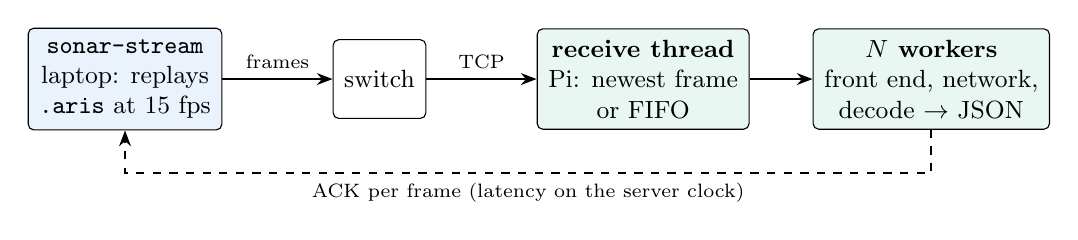
\begin{tikzpicture}[
  box/.style={draw, rounded corners=2pt, align=center, font=\small, minimum height=1.0cm, inner sep=4pt},
  arr/.style={-{Stealth[length=2mm]}, thick},
  node distance=0.8cm]
\node[box, fill=s1!10] (srv) {\textbf{\texttt{sonar-stream}}\\laptop: replays\\\texttt{.aris} at 15 fps};
\node[box, right=1.4cm of srv] (sw) {switch};
\node[box, right=1.4cm of sw, fill=s3!10] (rx) {\textbf{receive thread}\\Pi: newest frame\\or FIFO};
\node[box, right=of rx, fill=s3!10] (wk) {\textbf{$N$ workers}\\front end, network,\\decode $\to$ JSON};
\draw[arr] (srv) -- node[above, font=\scriptsize]{frames} (sw);
\draw[arr] (sw) -- node[above, font=\scriptsize]{TCP} (rx);
\draw[arr] (rx) -- (wk);
\draw[arr, dashed] (wk.south) -- ++(0,-0.55) -| node[pos=0.25, below, font=\scriptsize]{ACK per frame (latency on the server clock)} (srv.south);
\end{tikzpicture}
\caption{Streaming test. Each frame carries a sequence number and its
capture time; the client acknowledges every processed frame, and the
server computes capture-to-result latency on its own clock.}
\label{fig:stream}
\end{figure}

\paragraph{Protocol.} The emulator follows the idea of SeedLink, the
seismology streaming protocol. A client connects over TCP, names itself and
asks to start from the newest frame or from a sequence number. The server
sends each frame as a 64-byte header (sequence number, capture time, ARIS
geometry) followed by the beam data, and keeps the last 256 frames so that
a client can resume after a reconnect. Several clients can connect at once.
On the board, a receive thread hands frames to $N$ worker processes. Under
the \emph{latest} policy a free worker always takes the newest frame and
older waiting frames are dropped; under the \emph{queue} policy every frame
is processed in order and the delay grows when the board falls behind.
Latency is measured on the laptop's clock alone, from the frame's capture
time to the arrival of its acknowledgement, so clock offsets between the
machines do not enter. It includes the network transfer.

\paragraph{Correctness and network.} A 195-frame recording streamed to
each board gives output identical to the file-based run on every frame,
for both models and both boards. The laptop reached the Pi~4 at
941~Mbit/s (round trip 0.33~ms) and the Pi~2 at 94~Mbit/s, the limit of
its 100~Mbit/s port (0.85~ms). The stream needs at most 15~Mbit/s.

\paragraph{Sweeps.} One-minute runs over frame rates, worker counts and
both policies (Table~\ref{tab:sweep}) locate each board's limit. The Pi~4
sustains 30 frames/s on one worker and 120 frames/s on four, with results
about 23~ms after capture. The Pi~2 cannot keep up at 15 frames/s with one
or two workers; with three it does, but each result is about 143~ms after
capture. When a board falls behind, the queue policy lets the delay grow
to several seconds within a minute, while the latest policy keeps it near
one processing time and drops frames instead.

\begin{table}[H]
\centering
\caption{One-minute streaming runs of the deployed model. Latency from
capture to result, in ms.}
\label{tab:sweep}
\begin{tabular}{lrrlrr}
\toprule
Board & Rate (fps) & Workers & Policy & Processed fps (dropped) & Latency p50 / p95 \\
\midrule
Pi~4 & 15 & 1 & latest & 15.0 (0\,\%) & 22.6 / 23.0 \\
Pi~4 & 30 & 1 & latest & 30.0 (0\,\%) & 22.3 / 22.7 \\
Pi~4 & 60 & 1 & latest & 46.2 (23\,\%) & 30.8 / 38.3 \\
Pi~4 & 60 & 1 & queue & 52.0 (13\,\%) & 5825 / 6308 \\
Pi~4 & 60 & 2 & latest & 59.5 (0.8\,\%) & 22.7 / 23.1 \\
Pi~4 & 120 & 4 & latest & 119.9 (0.1\,\%) & 23.1 / 24.4 \\
\midrule
Pi~2 & 5 & 1 & latest & 5.0 (0\,\%) & 138.6 / 140.3 \\
Pi~2 & 15 & 1 & latest & 7.4 (51\,\%) & 178.2 / 207.5 \\
Pi~2 & 15 & 2 & latest & 14.8 (1.7\,\%) & 170.1 / 201.2 \\
Pi~2 & 15 & 2 & queue & 15.0 (0\,\%) & 714 / 1201 \\
Pi~2 & 15 & 3 & latest & 15.0 (0.1\,\%) & 143.0 / 147.1 \\
\bottomrule
\end{tabular}
\end{table}

\paragraph{Thirty-minute runs.} Each board then ran the deployed model at
15 frames/s for 30 minutes with the latest policy: the Pi~4 with one
worker and the Pi~2 with three (Table~\ref{tab:long},
Figure~\ref{fig:long}).

\begin{table}[H]
\centering
\caption{Thirty-minute runs at 15 frames/s (27\,000 frames), deployed
model, latest policy.}
\label{tab:long}
\begin{tabular}{lcc}
\toprule
 & Pi~4, 1 worker & Pi~2, 3 workers \\
\midrule
Frames processed & 26\,993 (15.0 fps) & 26\,939 (14.97 fps) \\
Dropped & 7 (0.03\,\%) & 61 (0.23\,\%) \\
Latency p50 / p95 / p99 (ms) & 29.9 / 31.9 / 47.3 & 144.6 / 149.0 / 160.1 \\
Network time per frame, mean (ms) & 20.4 & 127.2 \\
CPU load, mean & 9\,\% & 54\,\% \\
Temperature start $\to$ end (max) & 49.6 $\to$ 53.5\,$^\circ$C (56.9) & 39.5 $\to$ 46.5\,$^\circ$C (50.3) \\
Throttling & none & none \\
\bottomrule
\end{tabular}
\end{table}

Both boards keep up for the whole half hour. The fanless Pi~4 levels off
below 57\,$^\circ$C, far from its 80\,$^\circ$C limit, and never throttles. Its
latency in this run (29.9~ms) is 7~ms above the one-minute runs (22.6~ms)
because of a fault: during the first attempt the Pi~4's Ethernet link went
down and up 131 times in 12 minutes and came back at 100~Mbit/s instead of
1~Gbit/s, while the Pi~2 on the same switch was unaffected. The run was
repeated over the slower link, which adds about 8~ms to transfer each
105~KB frame; the processing time itself was unchanged (21.3~ms from
receipt to result in both). The cable or port of the Pi~4 is the likely
cause.

\begin{figure}[H]
\centering
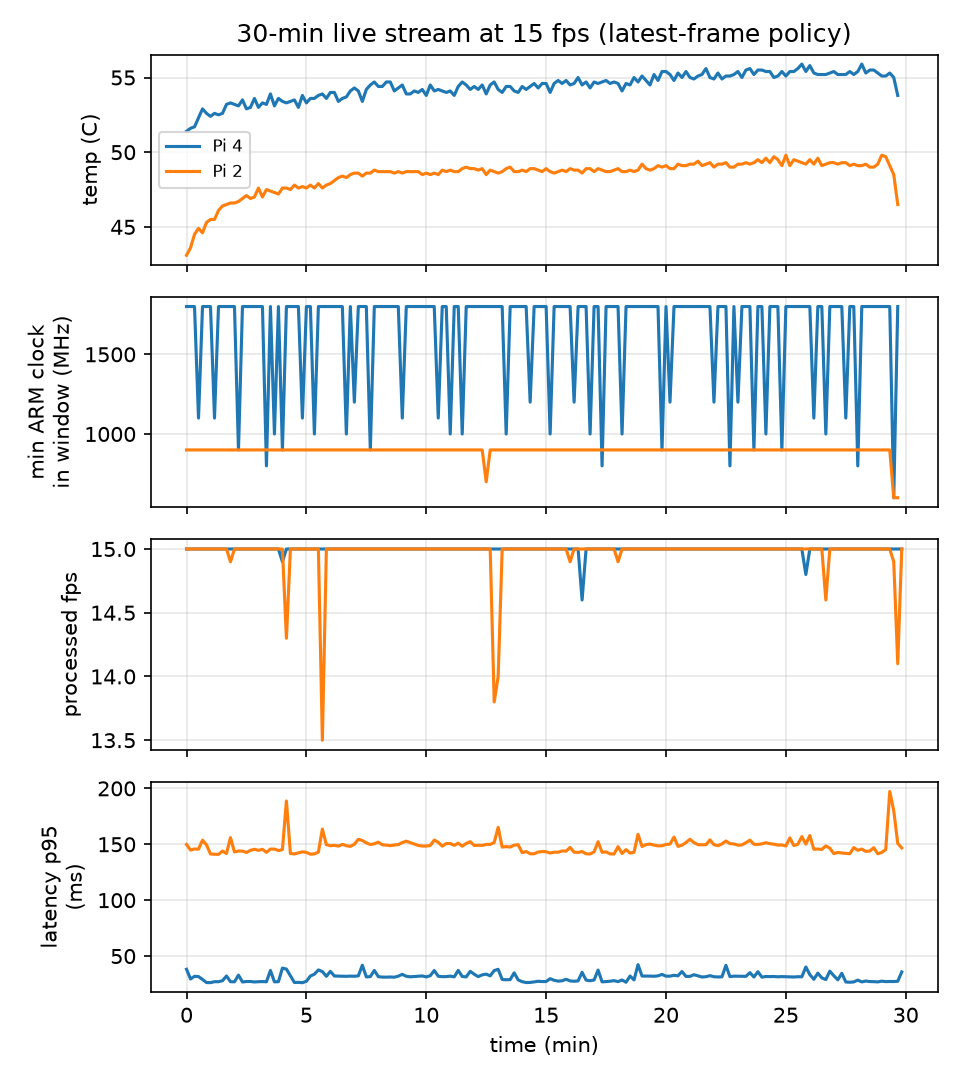
\includegraphics[width=0.66\textwidth]{fig/stream_long.png}
\caption{The thirty-minute runs, in 10-second windows: temperature, lowest
ARM clock in the window, frames processed per second and 95th-percentile
latency. The Pi~4 clock dips are the \texttt{ondemand} governor at 9\,\%
load, not throttling.}
\label{fig:long}
\end{figure}

Two points need care in reading these results. First, throughput is not
latency: one Pi~2 frame takes about 130~ms, two frame periods, so three
workers process frames in parallel and match the sensor's rate, but each
result is two frames old. A Pi~4-based vehicle would see the scene about
0.03~s late, a Pi~2-based one about 0.15~s late. Second, on the Pi~4 two
or four workers at 15 frames/s raise the 95th-percentile latency from 23
to about 40~ms, with 15--20\,\% of frames delayed. The cause was not
investigated; a likely candidate is an idle core that must first raise its
clock. One worker is the better setting on the Pi~4.

\paragraph{Bandwidth.} Keeping only detections with probability
$\geq 0.3$, each with its class, probability, box, range and bearing,
the result of a frame took 13~bytes on average for the deployed model and
52~bytes for \cfg{segdice} as compact JSON on these recordings (most frames
have no such detection and cost 2~bytes), against 53--124~KB for the raw
frame. These river recordings contain few objects, so scenes with many
objects would need more, but still a small fraction of the sonar data.

% ===========================================================================
\section{Discussion}

Closing the pipeline in C cost little and changed no result. Because the
front end reproduces the training resize bit for bit, every accuracy
figure measured on pre-resized frames holds for native fan images, and
the whole chain is reproduced exactly on a 64-bit and a 32-bit ARM
processor. The only new per-frame stage, the front end, takes 6\,\% of the
Pi~4's time per frame and 4\,\% of the Pi~2's; the network remains the
cost, so any further speed must come from it (a Pi~5 with dot-product
instructions, or several cores on one frame).

The Pi~2 shows that the runtime is not tied to a 64-bit board, but also
that kernel choices depend on the processor: the four-pixel kernel, the
right choice on the Pi~4, is the wrong one for the deployed model on the
Pi~2. The streaming test settles what the boards can do for the edge
task: the Pi~4 serves a 15 frames/s sonar from one core with an eighth of
its capacity, cool and with a 30~ms delay; the Pi~2 serves it only with
three cores and a 145~ms delay, which makes it a usable but marginal host.

The open part is the input. The raw polar path works on frames
back-projected from the dataset, with 0.6 points lost by the deployed
model, but nothing in this dataset tests it on what a sonar actually
records. The larger loss of the segmentation model on those frames
(4.8 points) suggests that its box branch, trained jointly with the mask,
is more sensitive to resampling; this is an observation on one fold, not
a measured cause. Training on the polar form itself does not help either
(Section~\ref{sec:polar}): the network is better off with the fan image.

% ===========================================================================
\section{Limitations}

\begin{itemize}
  \item \textbf{Input}: the fan-image path is tested exactly; the raw polar
        path only on frames back-projected from the fan images, because this
        dataset contains no raw ARIS data. The polar figures test the remap
        code, not performance on real recordings
        (Section~\ref{sec:dans} covers the separate test on raw recordings).
  \item \textbf{Real raw data, no accuracy}: the native ARIS recordings of
        Section~\ref{sec:dans} validate the raw path but have no labels,
        and come from a river rather than a tank. The detectors respond to
        riverbed texture as often without plastic as with it. Detection in
        such data would need labelled recordings and fine-tuning.
  \item \textbf{No metric scale}: the dataset does not document the range
        setting, so ranges for the tank data are in pixels.
  \item \textbf{One fold, one seed}: the end-to-end accuracy figures are
        for the fold-0 networks only; pooled five-fold figures are in the
        project report.
  \item \textbf{Segmentation model on polar input}: the 4.8-point loss was
        not investigated.
  \item \textbf{Pi~2}: one board, which needed a stronger power supply
        before it ran without under-voltage.
  \item \textbf{Emulated sensor}: the stream replays recordings from a
        laptop with the project's own protocol. A real ARIS sends its frames
        in UDP parts with its own protocol; that interface was not built.
  \item \textbf{Streaming runs}: one 30-minute run per board, deployed
        model only. The Pi~4's run used a 100~Mbit/s link after the link
        fault, which raised its latency by about 8~ms; it should be
        repeated at 1~Gbit/s after the cable is checked.
  \item \textbf{Polar input}: tested on back-projected frames with
        augmentations that are not faithful in polar form.
  \item \textbf{Energy}: not measured (no meter or power sensor).
\end{itemize}

% ===========================================================================
\section{Conclusions}

\begin{enumerate}
  \item The pipeline runs entirely in C, from the native fan image to
        boxes, classes, probabilities, a mask and range/bearing, in one
        network pass.
  \item On the 439-frame test fold its output on the Raspberry Pi~4 and
        the 32-bit Raspberry Pi~2 equals the laptop's on every frame (mAP
        63.81 for the deployed model, 57.09 with the mask).
  \item A frame takes \textbf{21.9~ms} on the Pi~4 (23.2~ms with the mask)
        and 128.5~ms on the Pi~2; the front end is 6\,\% and 4\,\% of it.
  \item The NEON kernel ports to 32-bit ARMv7 with exactness unchanged and
        is five times faster than scalar code there.
  \item Raw polar input works on real ARIS recordings: they are read,
        rendered and processed in 21.1~ms per frame on the Pi~4, with the
        same output as the laptop. The tank-trained detector does not
        transfer to that river data, and the data have no labels, so
        detection accuracy on raw sonar data is still unmeasured.
  \item On a live stream at 15 frames/s the fanless Pi~4 keeps up on one
        core for 30 minutes (0.03\,\% of frames dropped, results 30~ms after
        capture, at most 57\,$^\circ$C, no throttling). The Pi~2 keeps up on
        three cores with results 145~ms after capture.
  \item A network on the polar form of the data is 6.5 points worse at equal
        compute; the fan-image input stays.
\end{enumerate}

\section{Further work}

\begin{itemize}
  \item \textbf{Labelled field data}: a few hundred labelled frames from the
        DANS recordings would give the first accuracy figure on raw river
        data and a set for fine-tuning.
  \item \textbf{Energy}: an inline USB-C meter or an INA219/INA226 sensor
        for energy per frame at the 15 frames/s operating point.
  \item \textbf{Pi~4 at 1~Gbit/s}: repeat the 30-minute run after the cable
        is checked.
  \item \textbf{Live sonar}: the ARIS network protocol (discovery, commands,
        frames in UDP parts) is documented and was studied; implementing it
        would let the pipeline take frames from a real sonar.
\end{itemize}

% ===========================================================================
\appendix
\section{Reproduction}

\begin{small}
\begin{verbatim}
# export a model to its own directory; build and test
uv run python -m sonar_edge.export_c runs/small_360_segdice_cv_f0 \
    --out runtime/models/small_360_segdice
make -C runtime all test test-frontend                # shipped model
make -C runtime W=models/small_360_segdice all test   # another export
# run the pipeline
runtime/sonar-edge-run -m masks/ -o overlays/ frame.pgm ...  # fan or net size
runtime/sonar-edge-run --polar 128x439 frames.u8      # raw polar, or - for stdin
runtime/sonar-edge-run --aris [--fit metric|window] [--every N] rec.aris  # ARIS files
# back-projected polar frames of the dataset (synthetic; see Section 3)
uv run python -m sonar_edge.polar export OUT_DIR --beams 128 --samples 439
# live stream: server on the laptop, client on the board
runtime/sonar-stream --bind ADDR -p 5801 [--fps 15] rec.aris ...
runtime/sonar-edge-run --stream ADDR:5801 --policy latest --workers 1
# Raspberry Pi 2 (32-bit; Raspbian targets ARMv6 without NEON by default)
make CFLAGS="-std=c11 -O2 -Wall -Wextra -Werror -pedantic \
    -mcpu=cortex-a7 -mfpu=neon-vfpv4 -DSE_NEON_1PX" all
\end{verbatim}
\end{small}
Raw results are in the repository under \texttt{bench/}: \texttt{pi2/}
(Pi~2 benchmark), \texttt{e2e/} (end-to-end runs on both boards),
\texttt{dans/} (ARIS recordings; the download list and script fetch the
data from DANS), \texttt{stream/} (streaming) and \texttt{polar/} (polar
input). Technical notes are in \texttt{docs/}: M5 §3.7, M8, M9 and M10.

\end{document}
